%%%%%%%%%%%%%%%%%%%%%%%%%%%%%%%%%%%%%%%%%%%%%%%%%%%%%%%%%%%%%%%%%%%%%%%%%%%%%%%%
%2345678901234567890123456789012345678901234567890123456789012345678901234567890
%        1         2         3         4         5         6         7         8


\documentclass[a4paper, 10pt, conference] {article}        
                                                           

%\IEEEoverridecommandlockouts                              % This command is only
                                                          % needed if you want to
                                                          % use the \thanks command
%\overrideIEEEmargins
% See the \addtolength command later in the file to balance the column lengths
% on the last page of the document



% The following packages can be found on http:\\www.ctan.org
\usepackage{graphicx} % for pdf, bitmapped graphics files
\usepackage{caption}
\usepackage{float}
\usepackage{subcaption}
\usepackage{epsfig} % for postscript graphics files
\usepackage{mathptmx} % assumes new font selection scheme installed
\usepackage{times} % assumes new font selection scheme installed
\usepackage{amsmath} % assumes amsmath package installed
\usepackage{amssymb}  % assumes amsmath package installed
\usepackage[margin=1.5cm]{geometry}
\usepackage{mathtools}
\usepackage{enumerate}
\begin{document}
\date{}
\title{\LARGE \bf
Programming Assignment 2: Image denoising 
}

\author{ \parbox{5 in}{\centering Daniel Barmaimon \\
%         \thanks{*Use the $\backslash$thanks command to put information here}\\
         \ Advanced Image Analysis - Vibot Master Degree\\
         \ Heriot Watt University\\         
}}

\maketitle
%\thispagestyle{empty}
%\pagestyle{empty}









\section{Introduction}
The main purpose of this section is to create a bilateral filter. It should have certain weight depending in two basic features. The first feature will be the distance from the central pixel (the one to study) and the neighbours that are being considering. The second feature will be related with the difference in the intensity level between this pixel and its neighbours.

\section{Fundamentals}
Let's imagine an original image to be filtered with a bilateral filter
\begin{equation}
I_{0}(x,y) = I(x,y)
\end{equation} 
\begin{equation}
I_{n+1}(x,y) = \sum\limits_{i=-N}^N\sum\limits_{j=-N}^N w_{ij}I_{n}(x, y)/\sum\limits_{i=-N}^N\sum\limits_{j=-N}^N w_{ij} 
\end{equation}
\begin{equation}
w_{ij} = exp \left(- \frac {dist^2(X_{0}, X_{ij})}{2*\sigma^2_{d}} - \frac{\left| I(X_{0})-I(X_{ij})\right|^2}{2*\sigma^2_{r}}\right)
\end{equation}
In this filter \textit{N} is the length of half of the size of a square patch that will be consider as the neighbourhood of the pixel to study, and it is proportionally related to $\sigma_{d}$.
Several differences from the previous lab could be observed, the size of the neighbourhood won't be fixed, and the border to apply padding neither. The weight is depending in two exponential functions, allowing to consider with the most important influence the closer pixel and the intensity of such pixels. 
The last parameter will be the number of iterations, in the case, \textit{n}. 

 \begin{figure}[H]
 	%\centering
 	\begin{subfigure}{0.29\textwidth} 						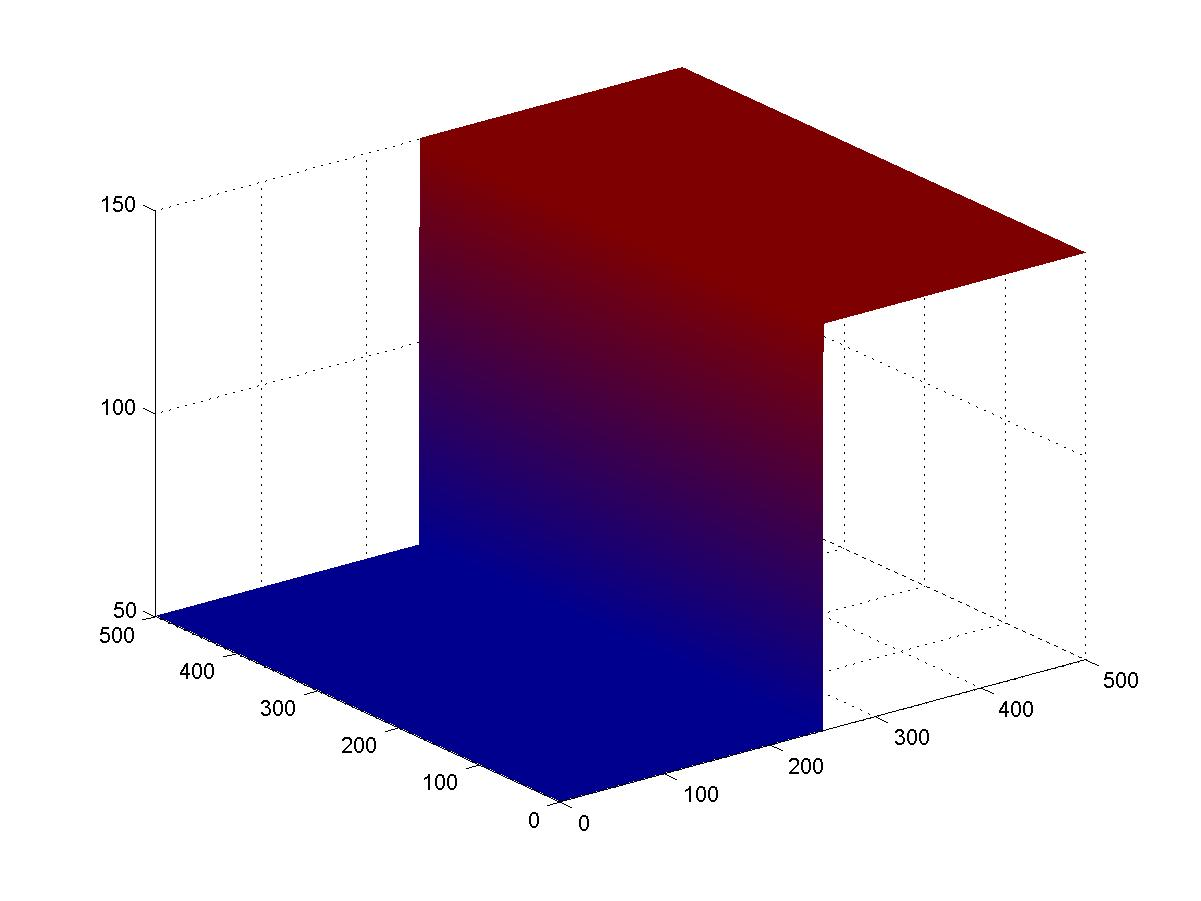
\includegraphics[scale=0.13]{original_1.JPG}
		\caption{Original}
	\end{subfigure}
	\begin{subfigure}{0.29\textwidth} 						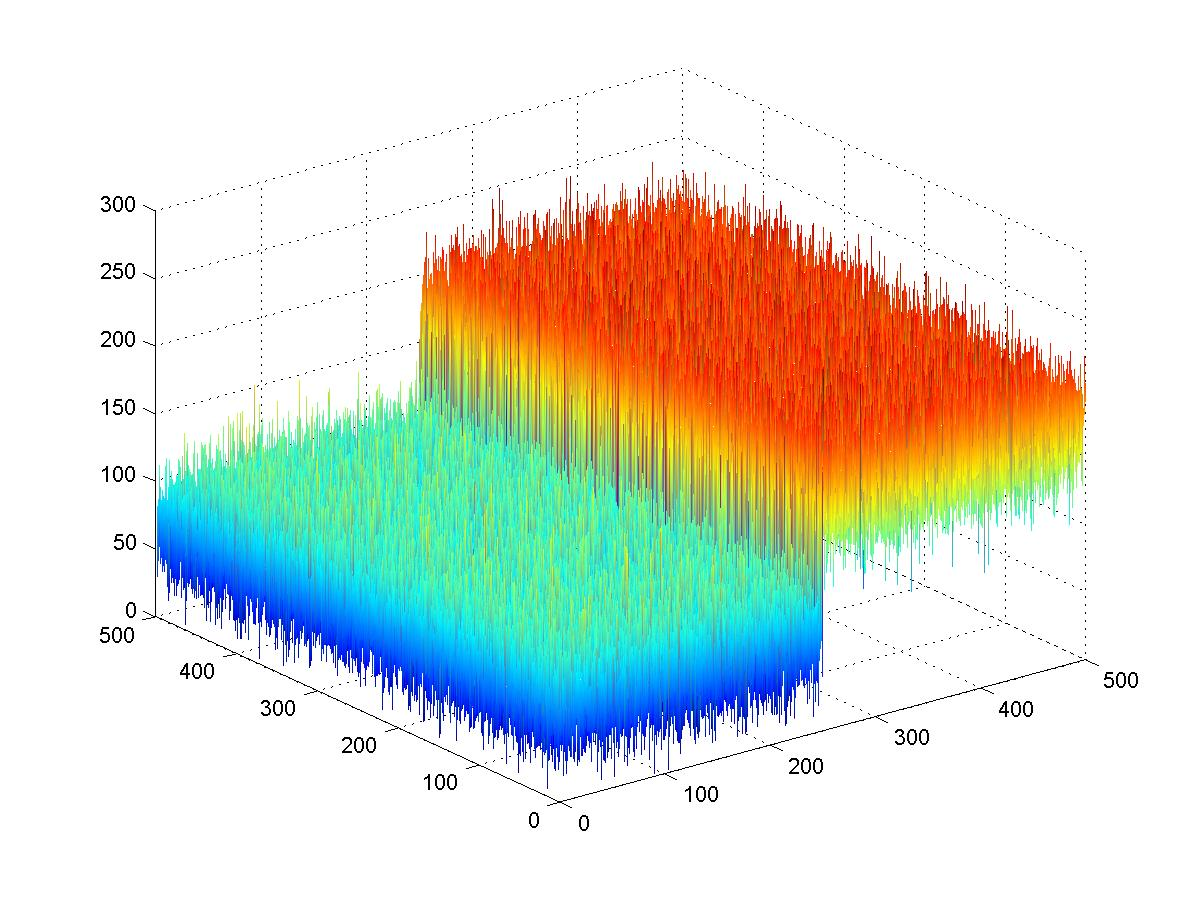
\includegraphics[scale=0.13]{noisy_1.JPG}
		\caption{Noisy}
	\end{subfigure}
	\begin{subfigure}{0.29\textwidth} 						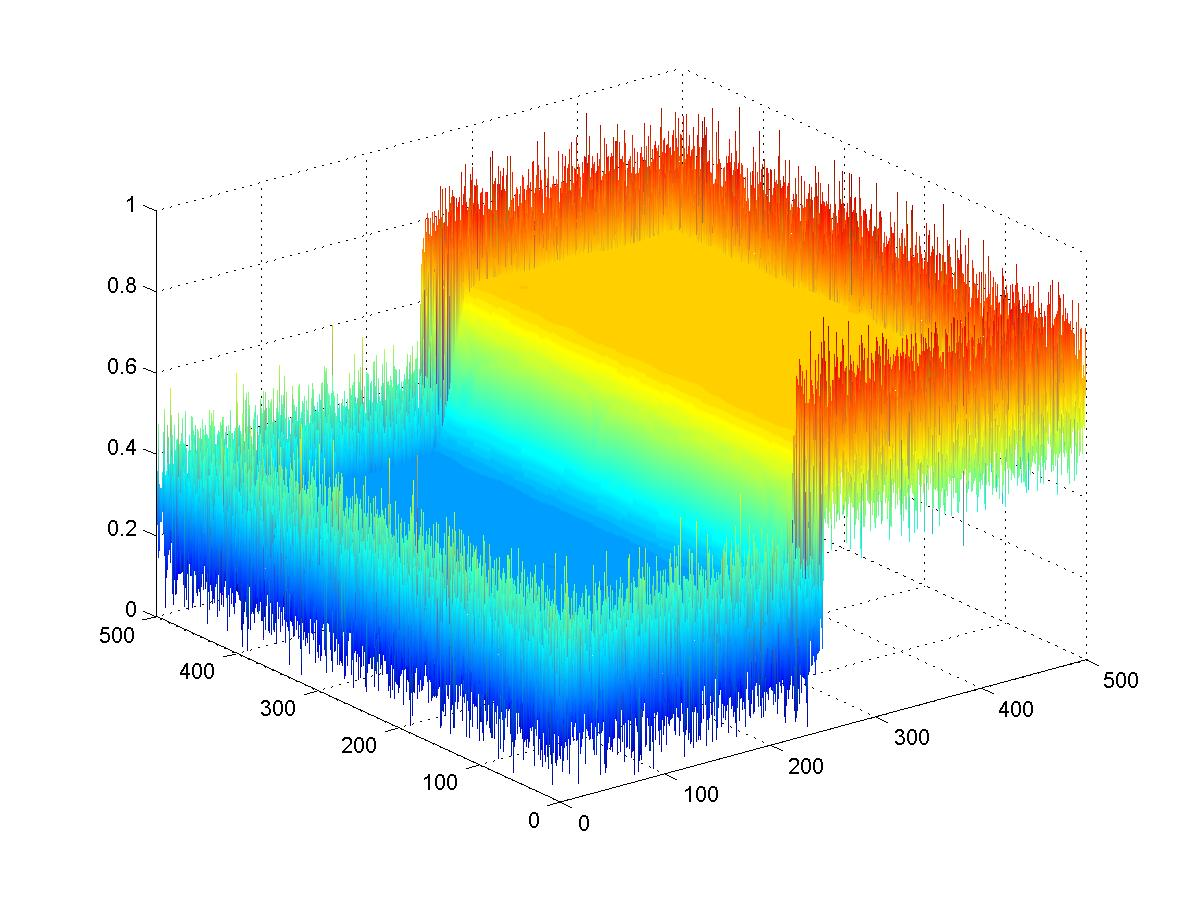
\includegraphics[scale=0.13]{filtered_1.JPG}
		\caption{Filtered}
	\end{subfigure}
	\caption{Synthetic image filtered with bilateral filter}
	\label{mesh}
\end{figure}
 

\section{Evaluation and analysis}
Once that the effect of the filter was checked over a synthetic image, would be nice to check how it works over a real image.
\begin{figure}[H]
	\centering
	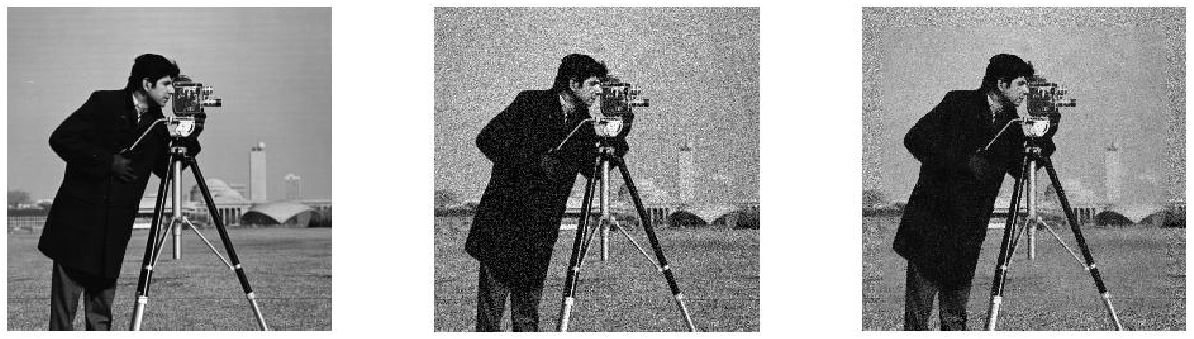
\includegraphics[width=1\textwidth]{camera_analysis.JPG} %
	\caption{Bilateral filter with $\sigma_{d}=8, \sigma_{r}=10, iterations = 1$}
	\label{camera}
\end{figure}
As it can be seen, the noise have been removed and edges are still remaining. It is also significant the size of the border, that of course, it not filtered. This padding problem could be partially solve mirroring the frame before applying the filter and cropping later on.    

\subsection{Analysis of $\sigma_{r}$ variation}
As the value of the parameter $\sigma_{r}$ is increased the filter will tend to be a regular average filter. This will be done by averaging with the same weight the neighbours that belong to the patch that contain as the central pixel the one that is being analysed. So the evolution of the blurring over the image could be seen in Fig.\ref{r} as this parameter changes.
\begin{figure}[H]
	\centering
	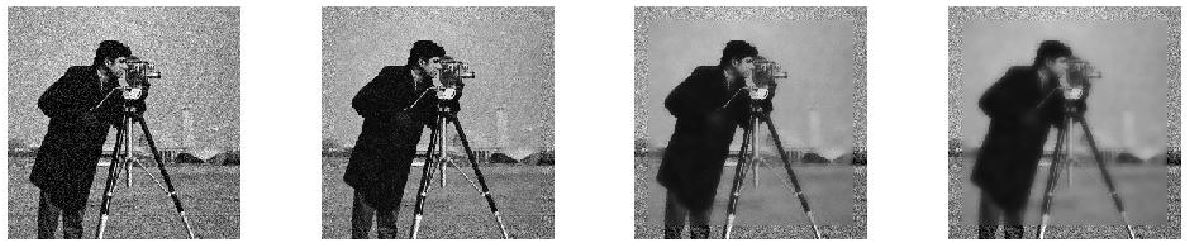
\includegraphics[width=1\textwidth]{sigmaR_analysis.JPG} %
	\caption{Bilateral filter with $\sigma_{d}=75; \sigma_{r}=4, 10, 20; iterations = 1$}
	\label{r}
\end{figure}


\subsection{Analysis of $\sigma_{d}$ variation}
The effect of increasing the parameter related with the distances will affect in a similar way to the filter. It should be remarked that the bigger this value is the more will affect to the borders of the image. This is shown in Fig.\ref{d}. Adjusting these two first parameter would be possible to give more weight to the distances or to the intensities.
\begin{figure}[H]
	\centering
	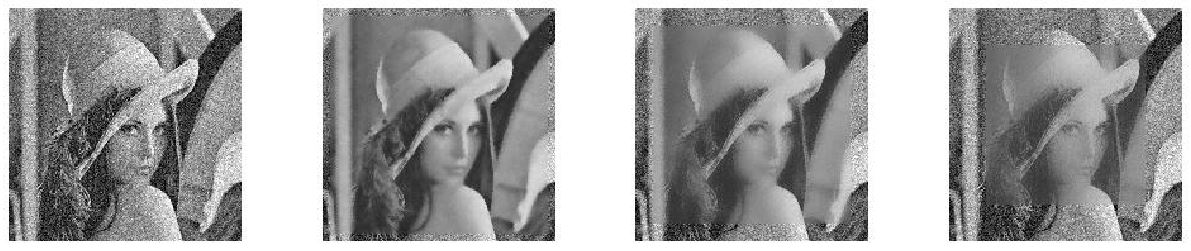
\includegraphics[width=1\textwidth]{sigmaD_analysis.JPG} %
	\caption{Bilateral filter with $\sigma_{d}=25, 75, 125; \sigma_{r}=4; iterations = 1$}
	\label{d}
\end{figure}

\subsection{Analysis of variation in the number of iterations}
One of the advantages of this filter is that works pretty will even with just one iteration. The computational time will increase drastically as we the number of iterations rise.
\begin{figure}[H]
	\centering
	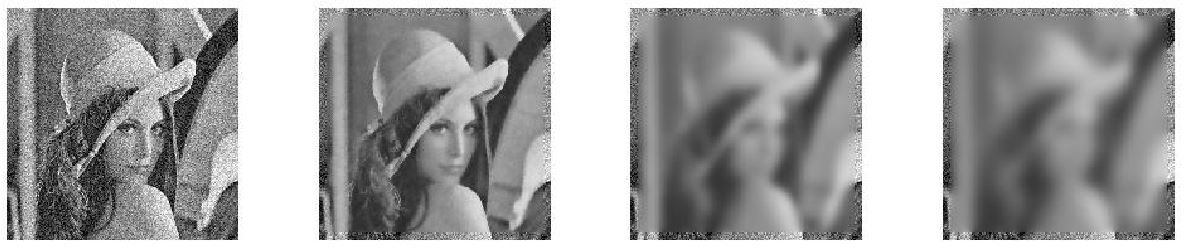
\includegraphics[width=1\textwidth]{iterations_analysis.JPG} %
	\caption{Bilateral filter with $\sigma_{d}=75; \sigma_{r}=4; iterations = 1, 10, 20$}
	\label{it}
\end{figure}


\subsection{Comparison of bilateral filter with non-local means filter}
Non-local means considers that each pixel \textit{x} will have as neighbours any pixel \textit{y} which neighbourhood is similar to the neighbourhood of \textit{x}.
\begin{equation}
I(x) = \frac{1}{C(x)}\int_{\omega}e^{-\frac{1}{h^2}\int_{\Re^{2}} G_{\textit{a}}(t)\lvert u(x+t) -u(y-t) \rvert^{2}dt} u(y)dy 
\end{equation}
where $G_{\textit{a}}$ is a Gaussian kernel of standard deviation \textit{a} and \textit{h} as a filtering parameter.

\begin{figure}[H]
	\centering
	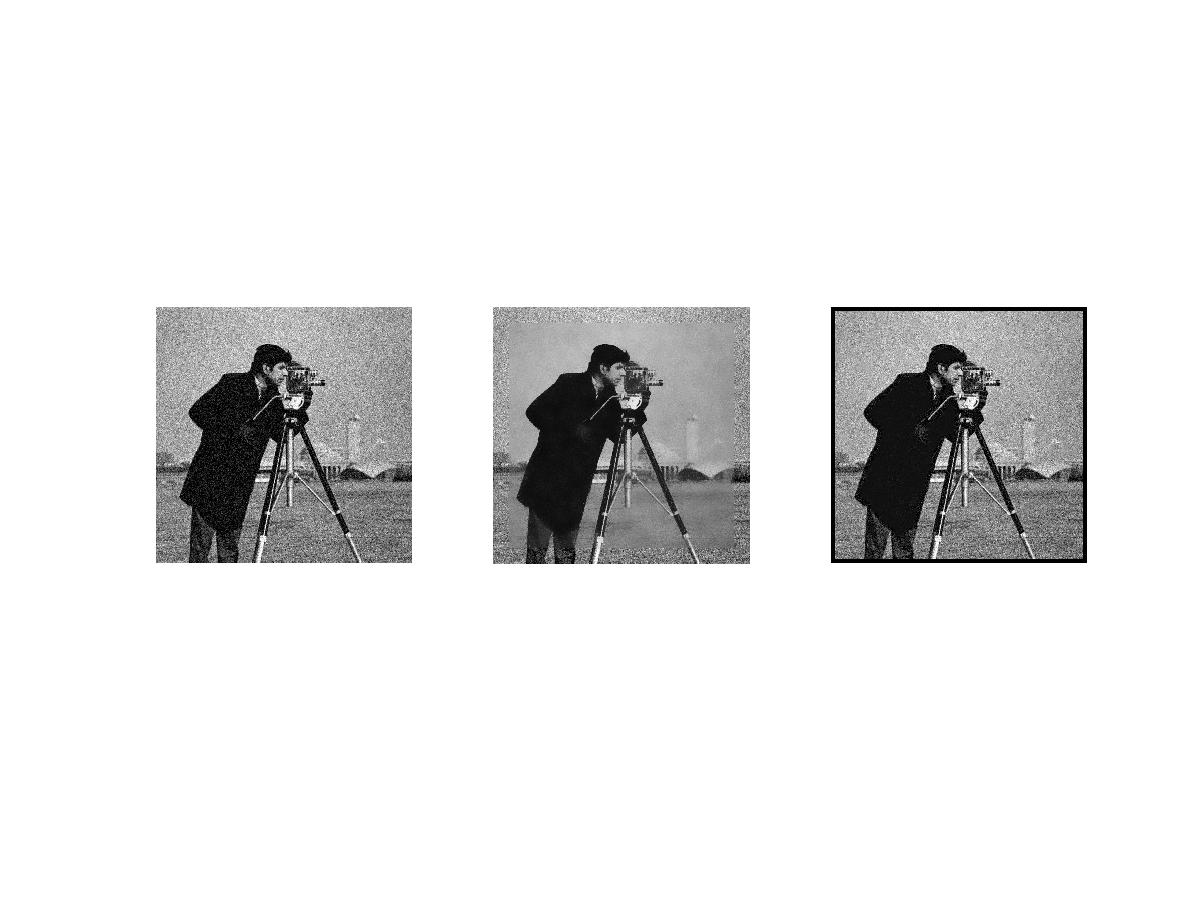
\includegraphics[width=1\textwidth]{bilateralVSnlmeans.JPG} %
	\caption{Original noisy image. Bilateral filter with $\sigma_{d}=50; \sigma_{r}=4; iterations = 1$. NLMeans with $N = 9$}
	\label{vs1}
\end{figure}
In Fig.\ref{vs1} a simpler version of the non-local means filter is used to compare with bilateral one. In a first instance is easy to check that the bilateral filter works much better in the preservation of the details (edges). The noise is also being removed in the non-local means filter. In the following pictures a deeper analysis will be performed. 
\begin{figure}[H]
	\centering
	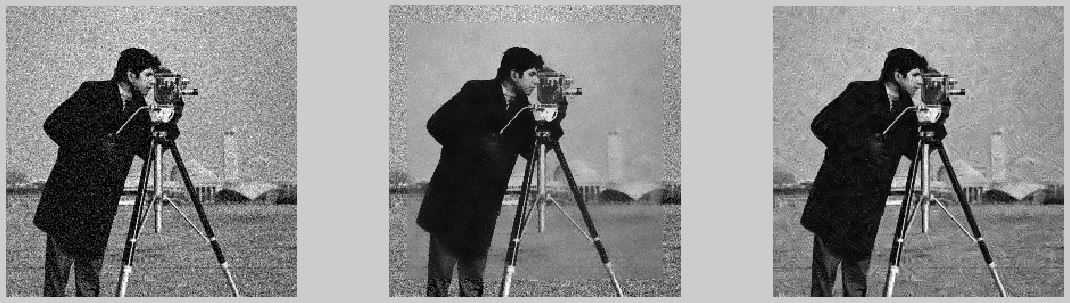
\includegraphics[width=1\textwidth]{bilateralVSnlmeans2.JPG} %
	\caption{Original noisy image. Bilateral filter with $\sigma_{d}=50; \sigma_{r}=4; iterations = 1$.  NLMeans with $N = 9$}
	\label{vs2}
\end{figure}
In this case a faster implementation of the non-local means has been used. In this case the edges are still better acquired by the bilateral filter but, non-local means seams to get more accurate grey levels.

Let analyse, Fig.\ref{noise_comp} the subtraction of the filtered images in both cases to the noisy image.
\begin{figure}[H]
	\centering
	
\includegraphics[width=1\textwidth]{noise_comparison.JPG} %
	\caption{Original noisy. Noise after bilateral filter; Noise after non-local means filter}
	\label{noise_comp}
\end{figure} 
 
The information about the edges has been lost much more in the bilateral filter. The only area that has better results is the camera, where are very small lines in different directions limiting zones with relatively high contrast. This noise should be almost similar if the parameters are properly set up. Summing up, it could be said that these filters are much better than regular averaging or Gaussian ones for denoising purposes. The edges information remain in the filtered image and most of the noise has been removed.
%First evaluation was made over the different values of \textit{k}. It will affect the weight, making the filter effect weaker as this value is increased. The effects could be appreciated in the image \ref{kanalysis}. 
%\begin{figure}[H]
%	\centering
%	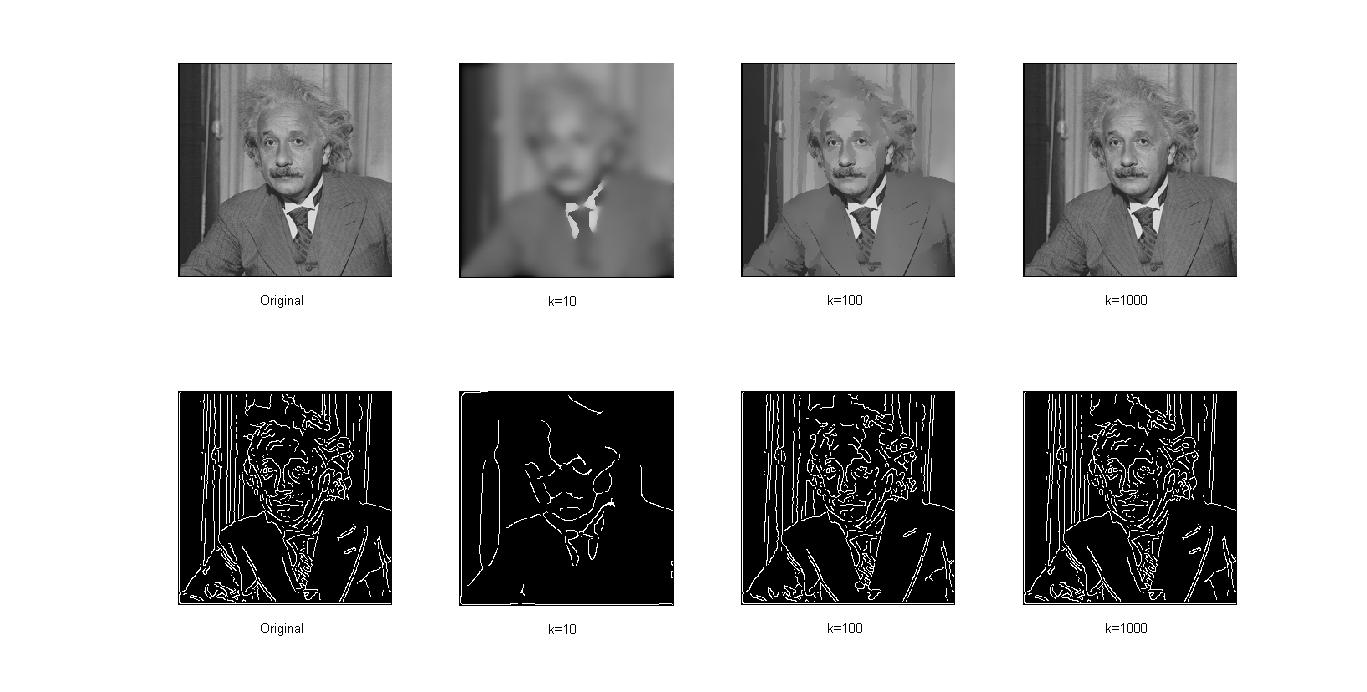
\includegraphics[width=1\textwidth]{analysis_einstein_k.JPG} %
%	\caption{Effects of varying \textit{k} over the image  for 50 iterations}
%	\label{kanalysis}
%\end{figure}
%
%It can be appreciated the differences in the two central images, where some areas have been smoothed while the edges could still been detected. An edge detection have been applied to the same images to check with detail the effects when \textit{k} varies. If \textit{k} is too big, the effects of the filter over the image are negligible. 
%
%\subsection{Analysis of \textit{n}, number of iterations}
%The number of iterations is the second parameter that should be set for a good performance of the filter. The bigger the number of iterations the more homogeneous will be the areas that compound the image, but also much more computational expensive.  
%\begin{figure}[H]
%	\centering
%	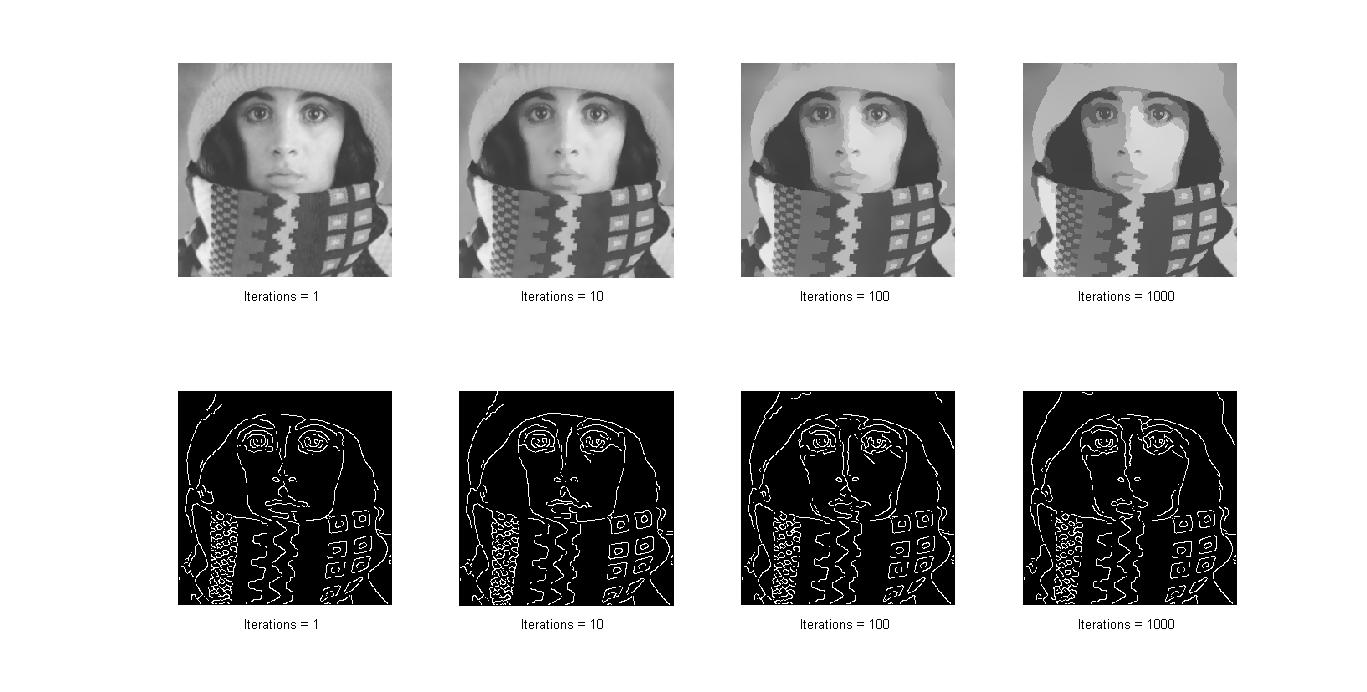
\includegraphics[width=1\textwidth]{analysis_trui_it.JPG} %
%	\caption{Effects of varying \textit{n}, nº of iterations for \textit{k}=100}
%	\label{itanalysis}
%\end{figure}
%In the Fig.\ref{itanalysis}, several experiments with different number of iterations were performed. For a deeper analysis a mesh plot over a small area of the same image will be shown in Fig.\ref{mesh}.
%
% \begin{figure}[H]
% 	\centering
% 	\begin{subfigure}{0.29\textwidth} 						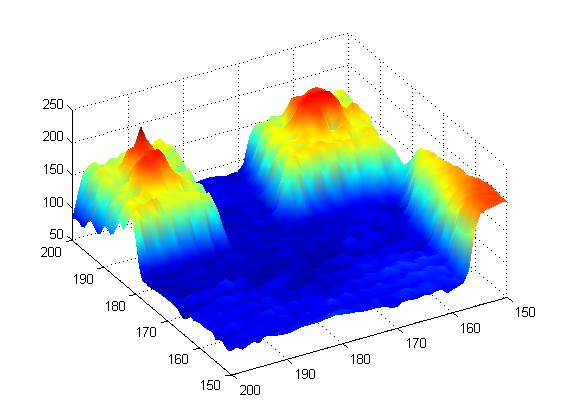
\includegraphics[scale=0.300]{mesh_original.JPG}
%		\caption{Original}
%	\end{subfigure}
%	\begin{subfigure}{0.29\textwidth} 						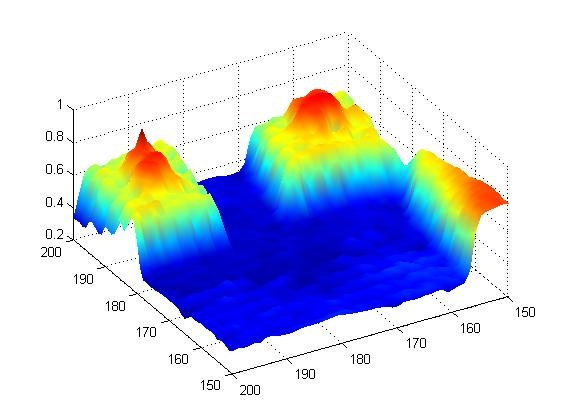
\includegraphics[scale=0.300]{mesh_solution1.JPG}
%		\caption{\textit{n}= 1 Iteration}
%	\end{subfigure}
%	\begin{subfigure}{0.29\textwidth} 						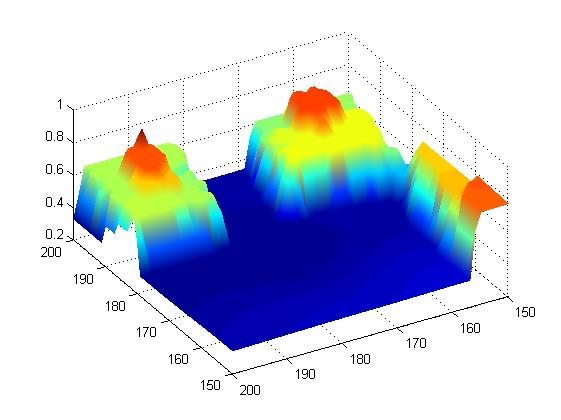
\includegraphics[scale=0.300]{mesh_solution3.JPG}
%		\caption{\textit{n}= 100 Iterations}
%	\end{subfigure}
%	\caption{Analysis with mesh grid plot for [125:200 ;125:200] for 'trui.tif'and \textit{k}=100}
%	\label{mesh}
%\end{figure}
%	
%As a simple example of how much the noise can be reduce and how good it could be for segmentation purposes the region growing algorithm was implemented over two different images, as is reflected in Fig.\ref{regionGrowing}
%\begin{figure}[H]
% 	\centering
% 	\begin{subfigure}{0.45\textwidth} 						
% 	\centering
% 	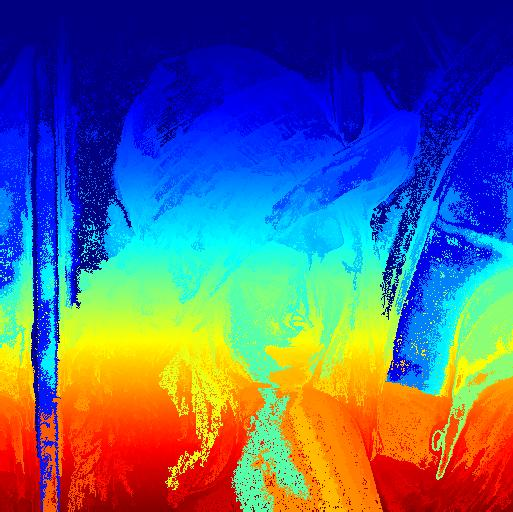
\includegraphics[scale=0.35]{original_segmented.JPG}
%		\caption{Original image}
%	\end{subfigure}
%	\begin{subfigure}{0.45\textwidth}
%	\centering
%	 						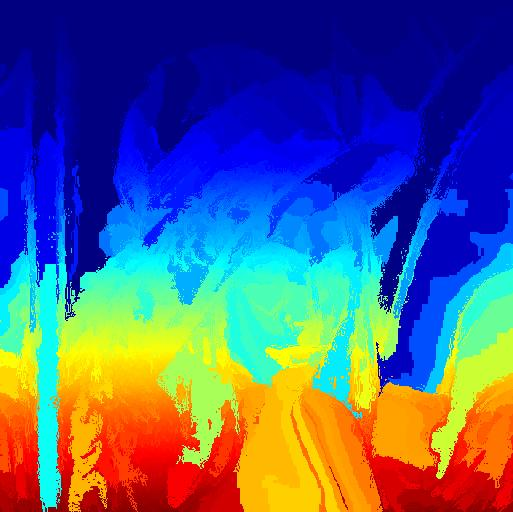
\includegraphics[scale=0.35]{filtered_segmented.JPG}
%		\caption{\textit{n}= 100 iterations, \textit{k}= 100}
%	\end{subfigure}
%	\caption{Region growing segmentation analysis}
%	\label{regionGrowing}
%\end{figure}
%
%%\begin{figure}[ht!]
%%  \centering
%%  \includegraphics[width=0.5\textwidth]{delta_qVsTime.jpg}
%%  \caption{Average time of computation versus step size}
%%  \label{timeVSstep}
%%\end{figure}
%
%The results shows a great reduction of the noise for the filtered image. The information of the edges is remaining but special care should be taken with the illumination sources and its effects over the filtered image.





% \begin{figure}[ht!]
% \centering
% \includegraphics[width=1\textwidth]{pseudoCode.JPG}
% \caption{Pseudo code for the A* algorithm representation}
% \label{pseudo}
% \end{figure}
%\clearpage 
%\section{Experiments}
%The implementation was quite straight forward using the pseudo code and having care to check the visibility in both directions. Until the path is found, the list of nodes that were checked and the ones to be considered are added into two different lists. The distances from last vertex, and the distance to the goal where checked and used as conditions to validate a new point of the path or to start to search in another branch.
%
%The results over two different environments are shown below. The environment is given by the vertices and the object they below to. The visibility for each environment is given. It is pretended to get to the last vertex from the first one by the shortest possible path.
%
%  \begin{figure}[ht!]
%  \begin{subfigure}{0.5\textwidth}
%  \centering
% \includegraphics{A.JPG}
%  \caption{Vertices coordintes and vertices for small environment}
%  \label{A}
%  \end{subfigure}
%  \begin{subfigure}{0.5\textwidth}
%  \centering
%  \includegraphics[scale=0.4]{small_environment.JPG}
%  \caption{Graphic plot of the results}
%  \label{resA}
%  \end{subfigure}\\
% 
%  \begin{subfigure}{0.5\textwidth}
%  \centering
%  \includegraphics[scale=0.8]{small_results.JPG}
%  \caption{List of visible combination for vertices}
%  \label{numA}
%  \end{subfigure}
%  \begin{subfigure}{0.5\textwidth}
%  \includegraphics[scale=0.8]{pathA.JPG}
%  \caption{Results for optimal path in small environment}
%  \label{pathA}
%  \end{subfigure}
%  \end{figure} 
%\clearpage
% \begin{figure}[ht!]
%  \begin{subfigure}{0.5\textwidth}
%  \centering
% \includegraphics{B.JPG}
%  \caption{Vertices coordintes and vertices for big environment}
%  \label{B}
%  \end{subfigure}
%  \begin{subfigure}{0.4\textwidth}
%  \includegraphics[scale=0.6]{big_environment.JPG}
%  \caption{Graphic plot of the results}
%  \label{resB}
%  \end{subfigure}\\
%
% 	\begin{tabular}{ c c c c}
%   	\begin{subfigure}{0.1\textwidth}
%   	        \centering
%   	         \includegraphics[scale=0.7]{big_results_01.JPG}
%   	          \label{numB1}
%   	\end{subfigure}&
%   	\begin{subfigure}{0.1\textwidth}
%   	  	        \centering
%   	  	         \includegraphics[scale=0.7]{big_results_02.JPG}
%   	  	         \label{numB2}
%   	  	\end{subfigure}&
%   	  	\begin{subfigure}{0.1\textwidth}
%   	  	  	        \centering
%   	  	  	         \includegraphics[scale=0.7]{big_results_03.JPG}
%   	  	  	          \label{numB3}
%   	  	  	\end{subfigure}& ~~~~~~~~~~~~~~~~~~~~~~~~~~~~~~ 
%   	  	  	\begin{subfigure}{\textwidth}
%   	  	  	  	  \includegraphics[scale=1]{pathB.JPG}
%   	  	  	  	  
%   	  	  	  	  \end{subfigure}
%  	\end{tabular}~~
%%  	\begin{subfigure}{0.5\textwidth}
%%  	  \includegraphics[scale=0.8]{pathB.JPG}
%%  	  \caption{Results for optimal path in big environment}
%%  	  \label{pathB}
%%  	  \end{subfigure}
%    	
%    	
%  
%  \end{figure} 
  

\begin{thebibliography}{99}
%%

\bibitem{c1}
'Advanced Image Analysis Notes', Alexander Belyaev, Heriot Watt University, 2014
%%
%%\bibitem{c3}
%%'Ultrasound Image Enhancement Based on Image Compounding' - Yair Kerner - Technion (Israel Institute of Technology) - Haifa - June 2004 
%%
%%\bibitem{c4}
%%'Physical Principles of General and Vascular Sonography' - Jim Baun - San Francisco, CA -March 2009
%%
%%\bibitem{c5}
%%'Physical Principles of General and Vascular Sonography' - Jim Baun - San Francisco, CA -March 2009
%%
%%\bibitem{c6}
%%'Image Formation and Image Processing in Ultrasound' - Jeffrey C. Bamber - Institute of Cancer Research and The Royal Marsden NHS Trust, Surrey, SM2 5PT
\end{thebibliography}

\end{document}
